\section*{Introduction}
When a positron is emitted inside a material, it can bind with an electron forming the so called Positronium. 

Positronium has two short lifetime bound states: the singlet para-Positronium~(p-Ps) and the triplet orto-Positronium~(o-Ps). They decay with the emission of two and three photons respectively, with a  life time 0.125~ns for the former and 142~ns for the latter. 
The aim of this report is to describe the experiment performed to study Positronium. The experiment has two main purposes:
\begin{itemize}
 \item Evaluate the decay ratio between o-Ps and p-Ps.
 \item Measure the temporal distribution for the two and three photons decays.
\end{itemize} 

\section*{Experimental Set Up}

To study the Positronium decay four inorganic NaI(Tl) cylindrical scintillators with 10~cm diameter and height were used~(see Fig.~\ref{Fig:Set_up}). Three of them were

\begin{wrapfigure}{L}{0.6\textwidth}
\centering
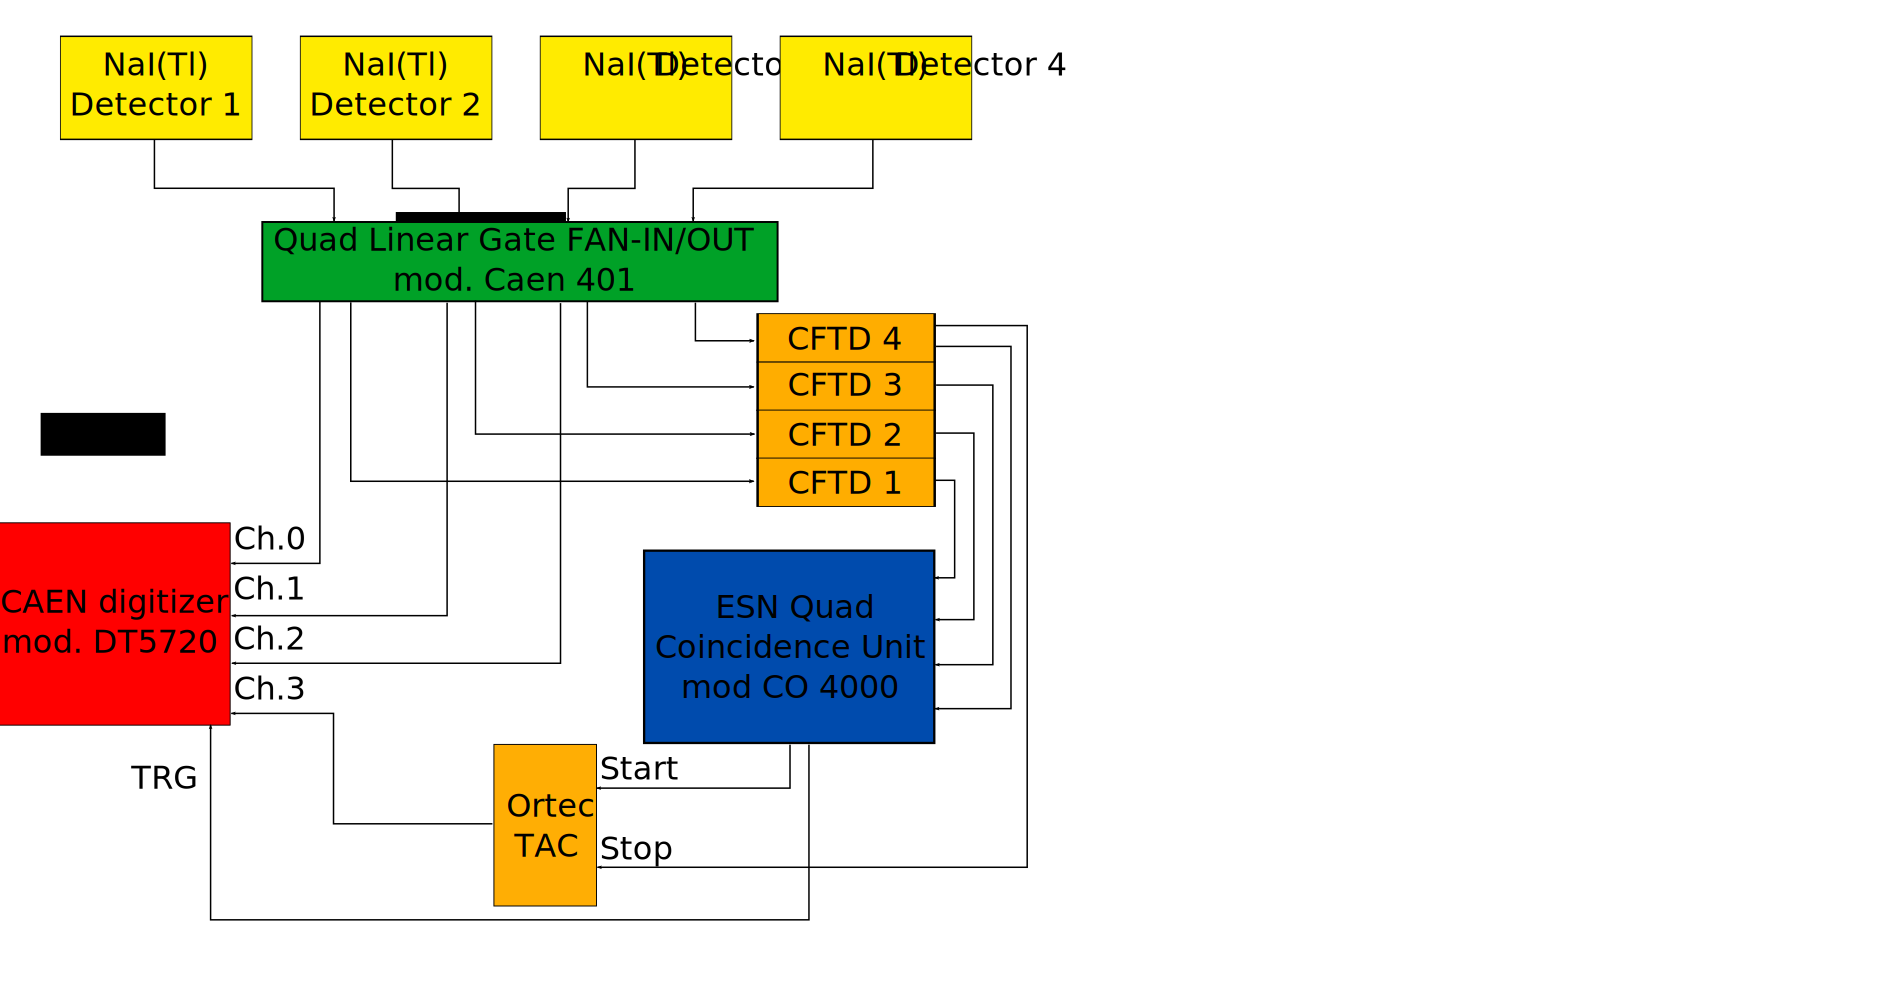
\includegraphics[width = 0.6\textwidth]{SetUp}
\caption{Electronic setup for the study of positronium decay.}
\label{Fig:Set_up}
\end{wrapfigure}
placed on a three arms goniometer centered on a $^{22}$Na $\gamma$-source, while the fourth was mounted vertically over it. The anode output of the detectors PMTs  were sent to a Quad Linear Gate FAN-IN/OUT mod. Caen 401 in order to split them. One output then was sent directly to a CAEN digitizer mod. DT5720, an ADC with a sampling rate of 250 Ms/s and a resolution of 12 bit, while the other ones were sent to a  CFTD module. The timing signals were needed to produce the coincidences between the detectors through a ESN Quad Coincidence Unit mod. CO 4000. These signals were sent then as trigger input for the ADC unit and as start signal for an Ortec TAC module,  to measure the time distribution of the positronium decays.

